
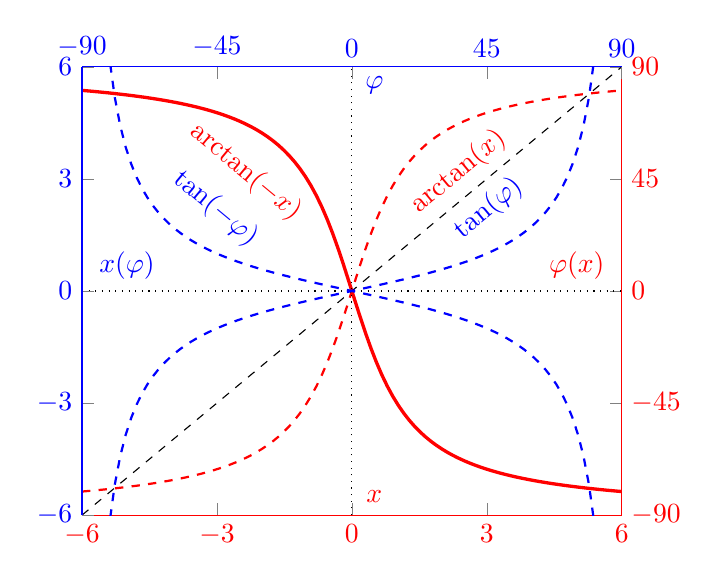
\begin{tikzpicture}
    % roughly same size as plot_tan_atan_mirror.tex
    % invisible boundbox
    %\draw[draw=black](-0.75,-0.5) rectangle (+7.5,+6.25);

    % plots with axis phi(omega)
    \begin{axis}[
        axis x line*=bottom,
        axis y line*=right,
        xmin = -6, xmax = +6, 
        xtick distance=3,
        ymin = -90, ymax = +90,
        %ytick distance=45,
        ytick={-90,-45,0,45,90},
        yticklabels={$-90\degree$, $-45\degree$, $0\degree$, $45\degree$, $90\degree$},
        domain=-6:6,
        samples=100,
        axis line style={red},
        every tick label/.append style={red},
        %every axis label/.append style ={red},% manual axis label within plot
    ]
        \addplot+[mark=none, color=red, very thick]{atan(-x)};
            %node[pos=0.15, below, sloped,yshift=-2pt]{$\arctan(-\varphi)$};
        \addplot+[mark=none, color=red, thick, dashed]{atan(x)};
            %node[pos=0.85, below, sloped,yshift=-2pt]{$\arctan(\varphi)$};

        % axis label
        \addplot+[mark=none] coordinates{(+0.5,-82.5)} node[red] {$x$};% x1
        \addplot+[mark=none] coordinates{(+0.5,+82.5)} node[blue]{$\varphi$};% x2
        \addplot+[mark=none] coordinates{(+5,+10)} node[red] {$\varphi(x)$};% y1
        \addplot+[mark=none] coordinates{(-5,+10)} node[blue]{$x(\varphi)$};% y2

        % extra axis for x=0 and for y=0 and diagonal (mirror line)
        \addplot+[mark=none, color=black, dotted]coordinates{(-6,0)(+6,0)};% x-axis
        \addplot+[mark=none, color=black, dotted]coordinates{(0,-90)(0,+90)};% y-axis
        \addplot+[mark=none, color=black, dashed]coordinates{(-6,-90)(+6,+90)}% diagonal
            node[pos=0.725, above, sloped, red]{$\arctan(x)$}% label
            node[pos=0.725, below, sloped, blue]{$\tan(\varphi)$};% label
        \addplot+[mark=none, draw=none, dashed]coordinates{(-6,+90)(+6,-90)}% diagonal
            node[pos=0.275, above, sloped, red]{$\arctan(-x)$}% label
            node[pos=0.275, below, sloped, blue]{$\tan(-\varphi)$};% label
    \end{axis}

    % plots with axis x2, f(x2)
    \begin{axis}[
        axis x line*=top,
        axis y line*=left,
        ymin = -6, ymax = +6,
        ytick distance=3,
        xmin = -90, xmax = +90,
        %xtick distance=45,
        xtick={-90,-45,0,45,90},
        xticklabels={$-90\degree$, $-45\degree$, $0\degree$, $45\degree$, $90\degree$},
        domain = -89.999:+89.999,
        samples=100,
        axis line style={blue},
        every tick label/.append style={blue},
        %every axis label/.append style ={blue},% manual axis label within plot
    ]
        \addplot+[mark=none, color=blue, thick, dashed, restrict y to domain=-10:10]{tan(x)};
            %node[pos=0.80, above, sloped, sloped,yshift=+2pt]{$\tan(x_2)$};
        \addplot+[mark=none, color=blue, thick, dashed, restrict y to domain=-10:10]{tan(-x)};
            %node[pos=0.20, above, sloped, sloped,yshift=+2pt]{$\tan(-x_2)$};

    \end{axis}
\end{tikzpicture}